
\section{Systematic Literature Search}
\label{sec:search}

\subsection{Search Strategy}
\label{subsec:search_strategy}

The literature search was conducted in January--February 2026 using the databases Google Scholar, ScienceDirect, Scopus, and ResearchGate, supplemented by citation graph exploration via Connected Papers to identify relevant works not captured by keyword search alone. Boolean search strings were constructed from combinations of the following keyword groups:

\begin{itemize}
    \item \textit{Application domain:} lubrication, lubrication condition monitoring, film thickness, lubrication degradation, lubricant starvation, grease condition, oil condition.
    \item \textit{Component:} ball bearing, rolling element bearing, roller bearing.
    \item \textit{Sensing modality:} vibration, acoustic emission, ultrasound, sound, microphone, thermal, infrared, electrical, capacitance, impedance, optical, magnetic, inductive.
    \item \textit{Signal processing:} signal processing, feature extraction, time domain, frequency domain, wavelet, machine learning, deep learning, neural network, regression, classification.
    \item \textit{Monitoring mode:} online, in-line, in-situ, condition monitoring.
\end{itemize}

\subsection{Inclusion and Exclusion Criteria}
\label{subsec:criteria}
\begin{table}[H]
\scriptsize
\centering
\renewcommand{\arraystretch}{1.4}
\setlength{\tabcolsep}{4pt}
\begin{tabularx}{\linewidth}{| >{\raggedright\arraybackslash}X | >{\raggedright\arraybackslash}X |}
\hline
\textbf{Inclusion criteria} & \textbf{Exclusion criteria} \\
\hline
Study concerns lubrication condition in rolling element bearings (including ball bearings, cylindrical roller bearings, tapered roller bearings, or slew bearings) & Study concerns journal bearings, thrust washers, or non-bearing lubricated contacts exclusively \\
\hline
Sensing method and signal processing approach are described in sufficient detail to assess the physical principle, processing operations, and output & Study provides only qualitative descriptions of sensing and processing without sufficient methodological detail \\
\hline
Monitoring is online, in-line, or in-situ (data collected during bearing operation) & Monitoring is exclusively offline (lubricant laboratory analysis without online data collection) \\
\hline
Study focuses on lubrication condition as the primary monitoring target (film thickness, viscosity, degradation, contamination, or regime) & Study concerns bearing fault detection or RUL estimation with no specific lubrication condition focus \\
\hline
English-language peer-reviewed journal papers, conference proceedings or manuals from industrial applications for LCM & Non-peer-reviewed sources (technical reports, white papers, patents) \\
\hline
\end{tabularx}
\caption{Inclusion and exclusion criteria for the systematic literature search.}
\label{tab:criteria}
\end{table}

\subsection{Search Results and PRISMA Flow}
\label{subsec:prisma}
\todo{Figure and text will be adjusted with updated numbers in the end.}
A total of 131 sources were initially identified through the literature search. After removal of duplicates across databases, 48 sources were identified as treating the topic of online or in-line LCM for rolling element bearings. Of these, 33 treated monitoring with active or invasive sensing methods and 20 treated passive and non-invasive sensing methods (some sources address both). All 48 are included as the primary basis for this review; the broader set of 131 sources provides supporting context for theoretical background, signal processing methodology, and industrial applications.

\begin{figure}[H]
\centering
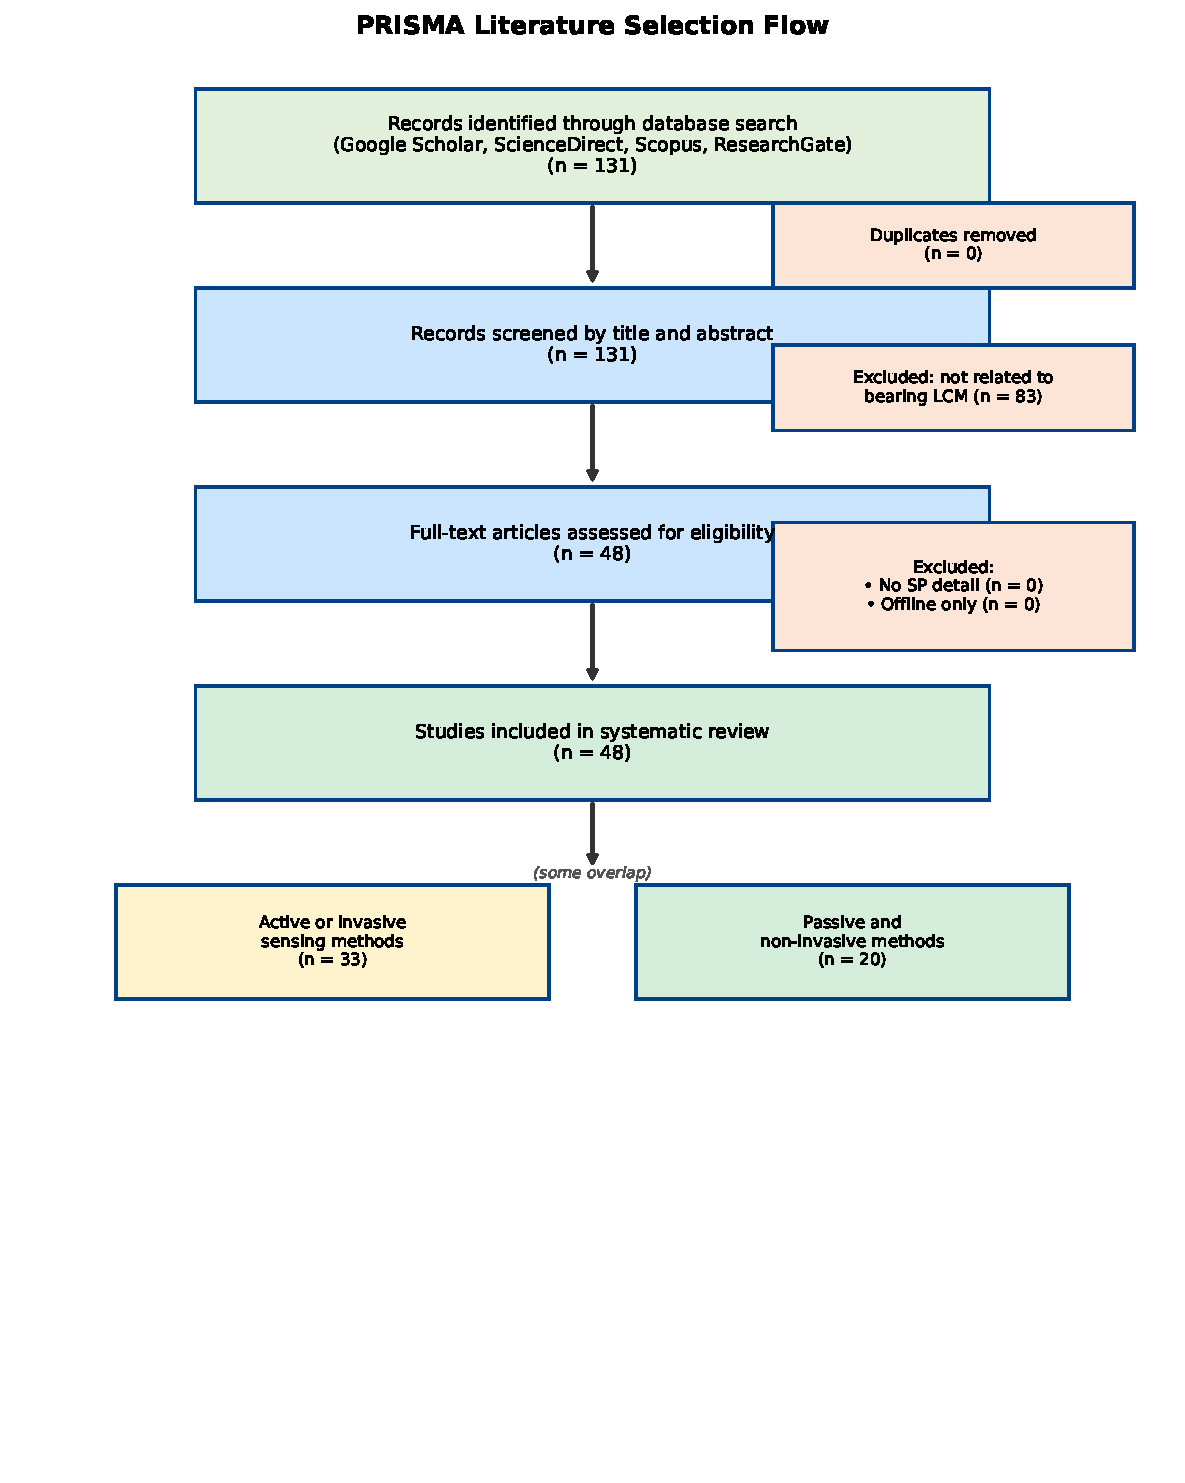
\includegraphics[width=0.65\textwidth]{figures/prisma_flow.pdf}
\caption{PRISMA-style literature selection flow diagram. Numbers reflect the search conducted in January--February 2026.}
\label{fig:prisma}
\end{figure}